\chapter{Experiments}

In this section the performed experiments are described and results of the
experiments are shown. The experiments were performed on the workstation
described in Section \ref{sec:setup}. All experiments were programmed in
Python and open-source software projects for the models and environment were
used extensively.

\section{Meta Reinforcement Learning}

The objective of the first experiment was to evaluate the adaptiveness and
reduce in retraining time with meta \rl. This is done using the meta \rl
offloading model, called \mrlco, proposed in \citeA{wang2020}. This model
required the data to be a \DAG in DOT format. For this, the Euro-Argo log data
was converted into these \DAG files. This process is described in Section
\ref{sec:data}. Running the experiments with the newly converted data required
modifications in the source code of \mrlco. In the \code{meta\_trainer.py}
file there was a list of directories containing 100 graph data files. This was
changed into the directories with our data. It was also possible to change
hyperparameters of the model in this source file, but this was not done in
this experiment.

% todo: hyperparameters wel of niet aangepast?
\begin{table}[htp!]
    \centering
    \caption{The average policy and environment execution time per run. The
    values are in seconds.}
    \label{table:exectime}
    \begin{tabular}{l|lccc}
        ID & Batch & Policy & Environment & Total\\ \hline
        1  & 1     & 4955   & 1907 & 6862\\
        2  & 1     & 4971   & 1907 & 6878\\
        3  & 2     & 5013   & 1822 & 6835
    \end{tabular}
\end{table}


The model was ran three times: first with their own data, then with the first
part of the converted Euro-Argo data and thereafter with the second part of
the converted Euro-Argo data. Each run consisted of 2,000 iterations in batch
sizes of 100. After each batch a TensorFlow checkpoint was saved on disk.
Every iteration it appended a row of data to a csv (comma separated value)
file. The following aspects of each iteration were saved:

\begin{itemize}[noitemsep]
    \item Iteration
    \item Number of trajectories
    \item Average reward
    \item Execution time:
        \begin{itemize}[noitemsep]
            \item Policy execution time
            \item Environment execution time
        \end{itemize}
    \item Return value:
        \begin{itemize}[noitemsep]
            \item Average return value
            \item Minimal return value
            \item Maximal return value
            \item Standard deviation of return value
            \item Average discounted return
        \end{itemize}
    \item Latency:
        \begin{itemize}[noitemsep]
            \item Average latency
            \item Average greedy latency
        \end{itemize}
\end{itemize}

\begin{figure}[htp!]
    \centering
    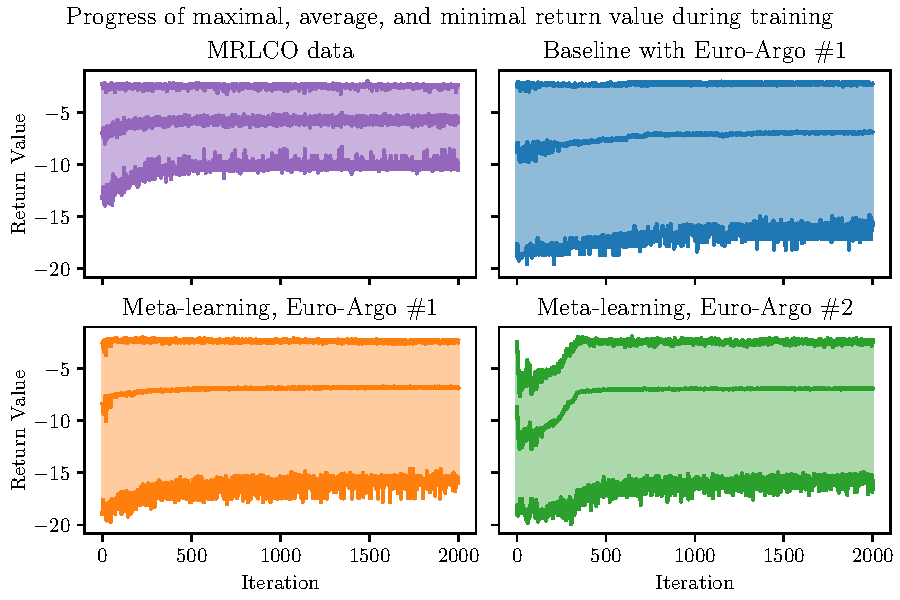
\includegraphics[width=\textwidth]{./fig/return.pdf}
    \caption{The progress of the return value during training. The upper line
    plots the maximal return value per iteration, the middle line the average
    return value and the lower line plots the minimal return value per
    iteration. The \#1 and \#2 are respectively the first and second batch of
    the Euro-Argo data.}
    \label{fig:return}
\end{figure}


The first run used 19 directories of 100 graph files. The reward in the last
iteration of training was $-5.42$. The average return value at the last
iteration was $-5.60$. For the second run the model was trained on 15
directories of 100 graph files, thus 1,500 graphs in total. The average reward
and average return in the last iteration where respectively $-6.74$ and
$-6.89$. The last run, on the other half of the Euro-Argo data, was also
performed on 1,500 graphs. The average reward and average return were $-6.97$
and $-6.93$ respectively. The maximal, minimal and average return value per
iteration are shown in Figure \ref{fig:return} and the progress of the average
reward during training is shown in Figure \ref{fig:rewards}. The model also
logged the execution time of the policy and environment. The average execution
times per run is listed in Table \ref{table:exectime}. There is little
difference in the execution times. The largest difference in Policy execution time
between \mrlco data and the second batch of the Euro-Argo data is 0.02889 and
the largest difference in environment execution time is 0.042484.

\begin{figure}[htp!]
    \centering
    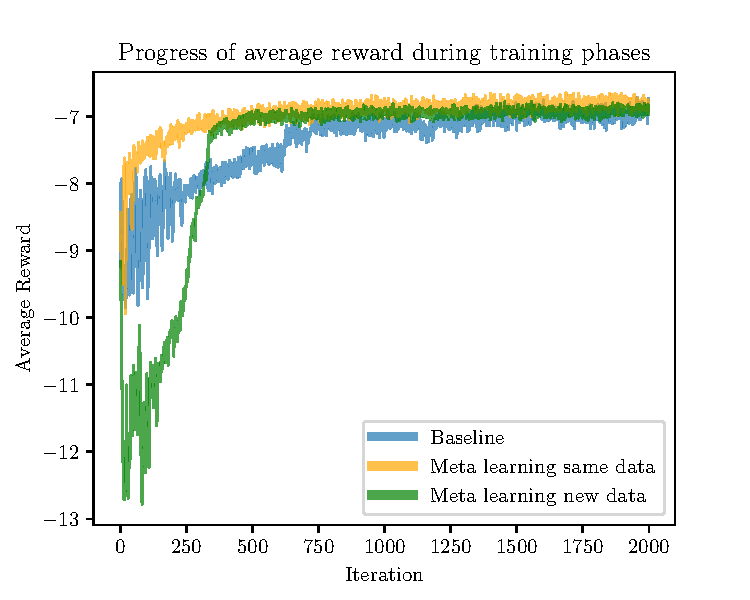
\includegraphics[width=.7\textwidth]{./fig/reward.pdf}
    \caption{The progress of average reward during training on \mrlco and
    Euro-Argo log data. The average reward on the \mrlco data seems to variate much
    more than on our data. The \mrlco data delivers a higher reward.}
    \label{fig:rewards}
\end{figure}


\section{OpenAI Gym}

The second experiments were done to evaluate multiple \rl algorithms as
schedulers. A side objective of this experiment was to have a good testbed for
future experiments. OpenAI's Gym was chosen for this because of its popularity
and simplicity. As described in Section \ref{sec:evaluation} and Section
\ref{sec:setup} OpenAI is a popular platform for creating, testing and
evaluating reinforcement learning models. The environment used in this
experiment is described in Section \ref{sec:taillard}. The \jss environment
(\code{JSSEnv}) in combination with the \code{keras-rl}
package\footlink{github.com/keras-rl/keras-rl} would allow us to experiment
with many different \rl algorithms and evaluate their performance as
scheduler. The \code{keras-rl} package currently supports \acrfull{dqn}
\cite{mnih2013}, Double \dqn \cite{hasselt2016}, Deep Deterministic Policy
Gradient \cite{lillicrap2015}, Continuous \dqn \cite{gu2016}, Cross-Entropy
Method \cite{szita2006}, Dueling network \dqn (Dueling \dqn) \cite{wang2016},
and Deep SARSA. Simulating the agent in the \jss environment required very
little code. First make the Gym environment, than define a neural network
(shown in Figure \ref{fig:neuralnetwork}), define a \rl agent, providing a
policy and the neural network for it, and lastly fit it on the environment.

\begin{figure}[htp!]
    \centering
    
\includegraphics[width=\textwidth]{./fig/nn.png}
    \caption{The \dnns used in the \rl models from \code{keras-rl}.}
    \label{fig:neuralnetwork}
\end{figure}


Starting the experiment, we first ran a FIFO scheduler (First-In-First-Out,
basically a queue) in the environment. The makespan after this run was 5724
and the final reward was -5.80 and the average reward was 0.40. After this
general Q-learning and the deep \rl algorithms mentioned above were tried.
There were no results due to various errors, which will be discussed in detail
in Section \ref{sec:discussion}.
